\documentclass[spanish,notitlepage,letterpaper,11pt]{article} % para artículo en castellano

\usepackage[utf8]{inputenc} % Acepta caracteres en castellano
\usepackage[T1]{fontenc} % font encoding
\usepackage[spanish]{babel} % silabea palabras castellanas
\usepackage[none]{hyphenat}
\usepackage{amsmath}
\usepackage{amsfonts}
\usepackage{amssymb}
\usepackage[colorlinks=true,urlcolor=blue,linkcolor=blue,unicode=true]{hyperref} % navega por el doc
\usepackage{graphicx}
\usepackage{geometry} % See geometry.pdf to learn the layout options.
\geometry{letterpaper}  % ... or a4paper or a5paper or ... 
%\geometry{landscape}  % Activate for for rotated page geometry
%\usepackage[parfill]{parskip} % Activate to begin paragraphs with an empty line rather than an indent
\usepackage{epstopdf}
\usepackage{fancyhdr} % encabezados y pies de pg
\usepackage{lineno}
\usepackage{float} % para usar [H] y forzar posicionamiento
%\linenumbers

\setcounter{tocdepth}{2} % profundidad del índice

\pagestyle{fancy} 
% \chead{\bfseries Taller de Distancias - Datos Reales (PM2.5)} 
\lhead{} % si se omite coloca el nombre de la seccion
% \rhead{26 de septiembre de 2025} 
\cfoot{Universidad Industrial de Santander} 
\rfoot{\thepage} 

%\voffset = -0.10in 
\setlength{\headheight}{28pt} % aumentar de 20pt a 28pt para evitar warnings/solapamiento
\setlength{\headsep}{12pt}    % espacio entre encabezado y el cuerpo del documento

% Configuración clara de fancyhdr (primero limpiar)
\pagestyle{fancy}
\fancyhf{} % borra cabeceras y pies previos

% Encabezado: izquierda, centro, derecha — usar tamaño small para evitar cortes
\fancyhead[L]{\small\itshape Taller de Distancias -- Datos Reales (PM2.5)}
\fancyhead[C]{} % dejar vacío o poner sección si lo deseas
\fancyhead[R]{\small 26 de septiembre de 2025}


\fancyfoot[C]{Universidad Industrial de Santander}
\fancyfoot[R]{\thepage}

% regla en el encabezado
\renewcommand{\headrulewidth}{0.5pt}
\renewcommand{\footrulewidth}{0.5pt}

\textheight = 8.0in 
\textwidth = 6.5in
\oddsidemargin = 0.in
\headheight = 20pt 
\headwidth = 6.5in
\renewcommand{\headrulewidth}{0.5pt}
\renewcommand{\footrulewidth}{0.5pt}
\DeclareGraphicsRule{.tif}{png}{.png}{`convert #1 `dirname #1`/`basename #1 .tif`.png}

\begin{document}
\title{Calibración de sensores IoT de PM2.5 usando datos reales}
\author{
\textbf{Juan David Mena Gamboa} \\ 
\textbf{Nicolás Santiago Espinosa Carrillo} \\
\textit{Escuela de Física, Universidad Industrial de Santander} \\ 
\textit{Bucaramanga, Colombia}}
\date{26 de septiembre de 2025}
\maketitle
\tableofcontents
\clearpage
% Nota: La tabla de contenidos se completa después de compilar LaTeX dos veces.

\begin{abstract}
Este trabajo aplica técnicas de calibración basadas en distancias euclidianas para mejorar la precisión de sensores IoT de material particulado fino (PM2.5) utilizando datos reales. Se analizaron 547 pares de mediciones sincronizadas entre estaciones de referencia (AMB) y sensores de bajo costo durante 2019.

La metodología empleó promedios móviles con ventanas de 0.5 a 6.0 horas para calcular distancias euclidianas entre las series. La ventana óptima de 6.0 horas minimizó la distancia (8.3890) y permitió un ajuste lineal con $R^2 = 0.7144$. El modelo de calibración resultante fue: \(f = 0.4389 \cdot \hat{f} + 4.3893\), con RMSE = 2.6369~$\mu\mathrm{g}/\mathrm{m}^3$.

El análisis de validez demostró que el modelo es confiable (tolerancia 25\%) para concentraciones del sensor IoT entre 2.01 y 38.10~$\mu\mathrm{g}/\mathrm{m}^3$. Se determinó que 200 pares de datos son suficientes para entrenamiento manteniendo capacidad predictiva. Los resultados evidencian la viabilidad de calibrar sensores de bajo costo usando métricas de distancia y ajustes lineales simples.
\end{abstract}

\section{Introducción}
En este reporte aplicamos el Taller de Distancias a datos reales de concentración de material particulado fino (PM2.5), calibrando un sensor IoT de bajo costo frente a estaciones de referencia (AMB). Presentamos el cálculo de distancias euclidianas entre promedios móviles, la selección de la ventana óptima, el ajuste de un modelo lineal y el análisis del alcance de validez.

\section{Metodología}
\label{Metodologia}
Se cargaron datos de referencia desde estaciones AMB (archivo Excel) y datos del sensor IoT desde múltiples archivos CSV (2019+). Las series fueron sincronizadas por tiempo real emparejando mediciones dentro de una tolerancia de 1 hora y luego se calcularon promedios móviles sobre una ventana común. La distancia euclidiana entre promedios permitió comparar ambas fuentes.

Se evaluaron ventanas entre 0.5 y 6.0 horas. El mejor ancho de ventana se seleccionó minimizando la distancia promedio. Con la ventana óptima se ajustó un modelo lineal por mínimos cuadrados de la forma $f(\xi_j)=\alpha\,\hat f(\xi_j)+\beta$.

\subsection{Resumen de datos y parámetros}
\begin{table}[h]
  \centering
\begin{tabular}{l|l}
\hline
Puntos de referencia & 547 \\ \hline
Puntos del sensor & 547 \\ \hline
Rango temporal (ref) & 0.00 -- 546.00 horas \\ \hline
Rango temporal (IoT) & 0.00 -- 546.00 horas \\ \hline
Rango PM2.5 (ref) & 3.20 -- 28.10~$\mu\mathrm{g}/\mathrm{m}^3$ \\ \hline
Rango PM2.5 (IoT) & 0.33 -- 45.17~$\mu\mathrm{g}/\mathrm{m}^3$ \\ \hline
Ventana óptima & 6.00 h \\ \hline
Distancia mínima & 8.3890 \\ \hline
Modelo lineal & $f=0.4389\,\hat f + 4.3893$ \\ \hline
$R^2$ & 0.7144 \\ \hline
RMSE & 2.6369 \\ \hline
Tolerancia & 25\% \\ \hline
Intervalo válido (IoT) & [2.01, 38.10]~$\mu\mathrm{g}/\mathrm{m}^3$ \\ \hline
\end{tabular}
\caption{Resumen de los conjuntos y parámetros obtenidos.}
\label{TablaResumen}
\end{table}

\section{El experimento y los resultados}
\label{Resultados}
Se evaluaron 20 valores de ventana entre 0.5 y 6.0 horas. La distancia euclidiana disminuyó con el aumento del ancho de ventana y alcanzó un mínimo de 8.3890 en 6.00 horas, que se tomó como ventana óptima. Con esta ventana, el ajuste lineal produjo la relación $f=0.4389\,\hat{f} + 4.3893$, con $R^2=0.7144$ y RMSE $=2.6369$~$\mu\mathrm{g}/\mathrm{m}^3$.

A continuación se analizan en detalle las cuatro subfiguras de la Figura~\ref{FiguraResultados} (todas generadas a partir de las mismas series sincronizadas):

\begin{itemize}
  \item \textbf{Panel (a) — Series originales (panel superior izquierdo).} Muestra las series temporales crudas de la estación AMB (azul) y del sensor IoT (rojo). Se observa que el sensor IoT presenta mayor varianza y picos puntuales (ruido y posibles lecturas erróneas), mientras que la estación AMB exhibe una curva más suave. Además existe un sesgo sistemático: en muchas regiones el IoT reporta valores mayores que la AMB, y en otras menores; esto justifica el uso de un suavizado y de un ajuste lineal con término independiente.

  \item \textbf{Panel (b) — Promedios móviles (panel superior derecho).} Al aplicar promedios móviles (ventana óptima 6.0 h) las series quedan suavizadas y las oscilaciones de alta frecuencia se atenúan. Esto facilita visualizar la tendencia de fondo y reduce el impacto de picos aislados en el cálculo de la distancia. Nótese que el suavizado reduce la discrepancia instantánea entre ambas series pero mantiene la diferencia sistemática que motiva la calibración.

  \item \textbf{Panel (c) — Ajuste del modelo (panel inferior izquierdo).} Aquí se grafican los pares sincronizados $(\hat f(\xi_j),f(\xi_j))$ y se muestra la recta de mínimos cuadrados. La pendiente encontrada ($\approx0.4389$) menor que 1 indica que el sensor IoT tiende a subestimar las variaciones reales en magnitud relativa; el intercepto positivo ($\approx4.3893$) sugiere un sesgo aditivo. El coeficiente de determinación $R^2=0.7144$ indica que el modelo lineal explica la mayor parte de la variabilidad entre promedios móviles, aunque persisten residuos apreciables en concentraciones altas.

  \item \textbf{Panel (d) — Optimización de la ventana móvil (panel inferior derecho).} Se muestra la distancia euclidiana calculada para distintas ventanas. La distancia decrece con el aumento de la ventana hasta alcanzar un mínimo en 6.0 h (distancia = 8.3890). Esto indica que el suavizado de 6 h logra el mejor emparejamiento entre fuentes bajo la métrica euclidiana considerada; ventanas mayores no aportan mejoras significativas.
\end{itemize}

Como se observa en la Tabla~\ref{TablaResumen}, el modelo muestra buen poder explicativo con un coeficiente de determinación superior al 71\%. La pendiente de 0.4389 indica que el sensor IoT subestima sistemáticamente las concentraciones, mientras que el intercepto de 4.3893~$\mu\mathrm{g}/\mathrm{m}^3$ sugiere un sesgo constante.

Definiendo una tolerancia del 25\%, el intervalo de validez sobre el eje del sensor fue $[2.01, 38.10]$~$\mu\mathrm{g}/\mathrm{m}^3$. Este rango cubre la mayoría de las concentraciones observadas, demostrando la aplicabilidad práctica del modelo. Usando una partición simple entrenamiento/validación, se encontró un tamaño mínimo de entrenamiento de 200 pares que mantiene capacidad predictiva en validación dentro del intervalo indicado.

La Figura~\ref{FiguraResultados} ilustra claramente la evolución temporal de ambas series, la efectividad del suavizado mediante promedios móviles, y la calidad del ajuste lineal. El panel de optimización confirma que ventanas mayores a 6 horas no mejoran significativamente la sincronización.

\begin{figure}[H]
\centering
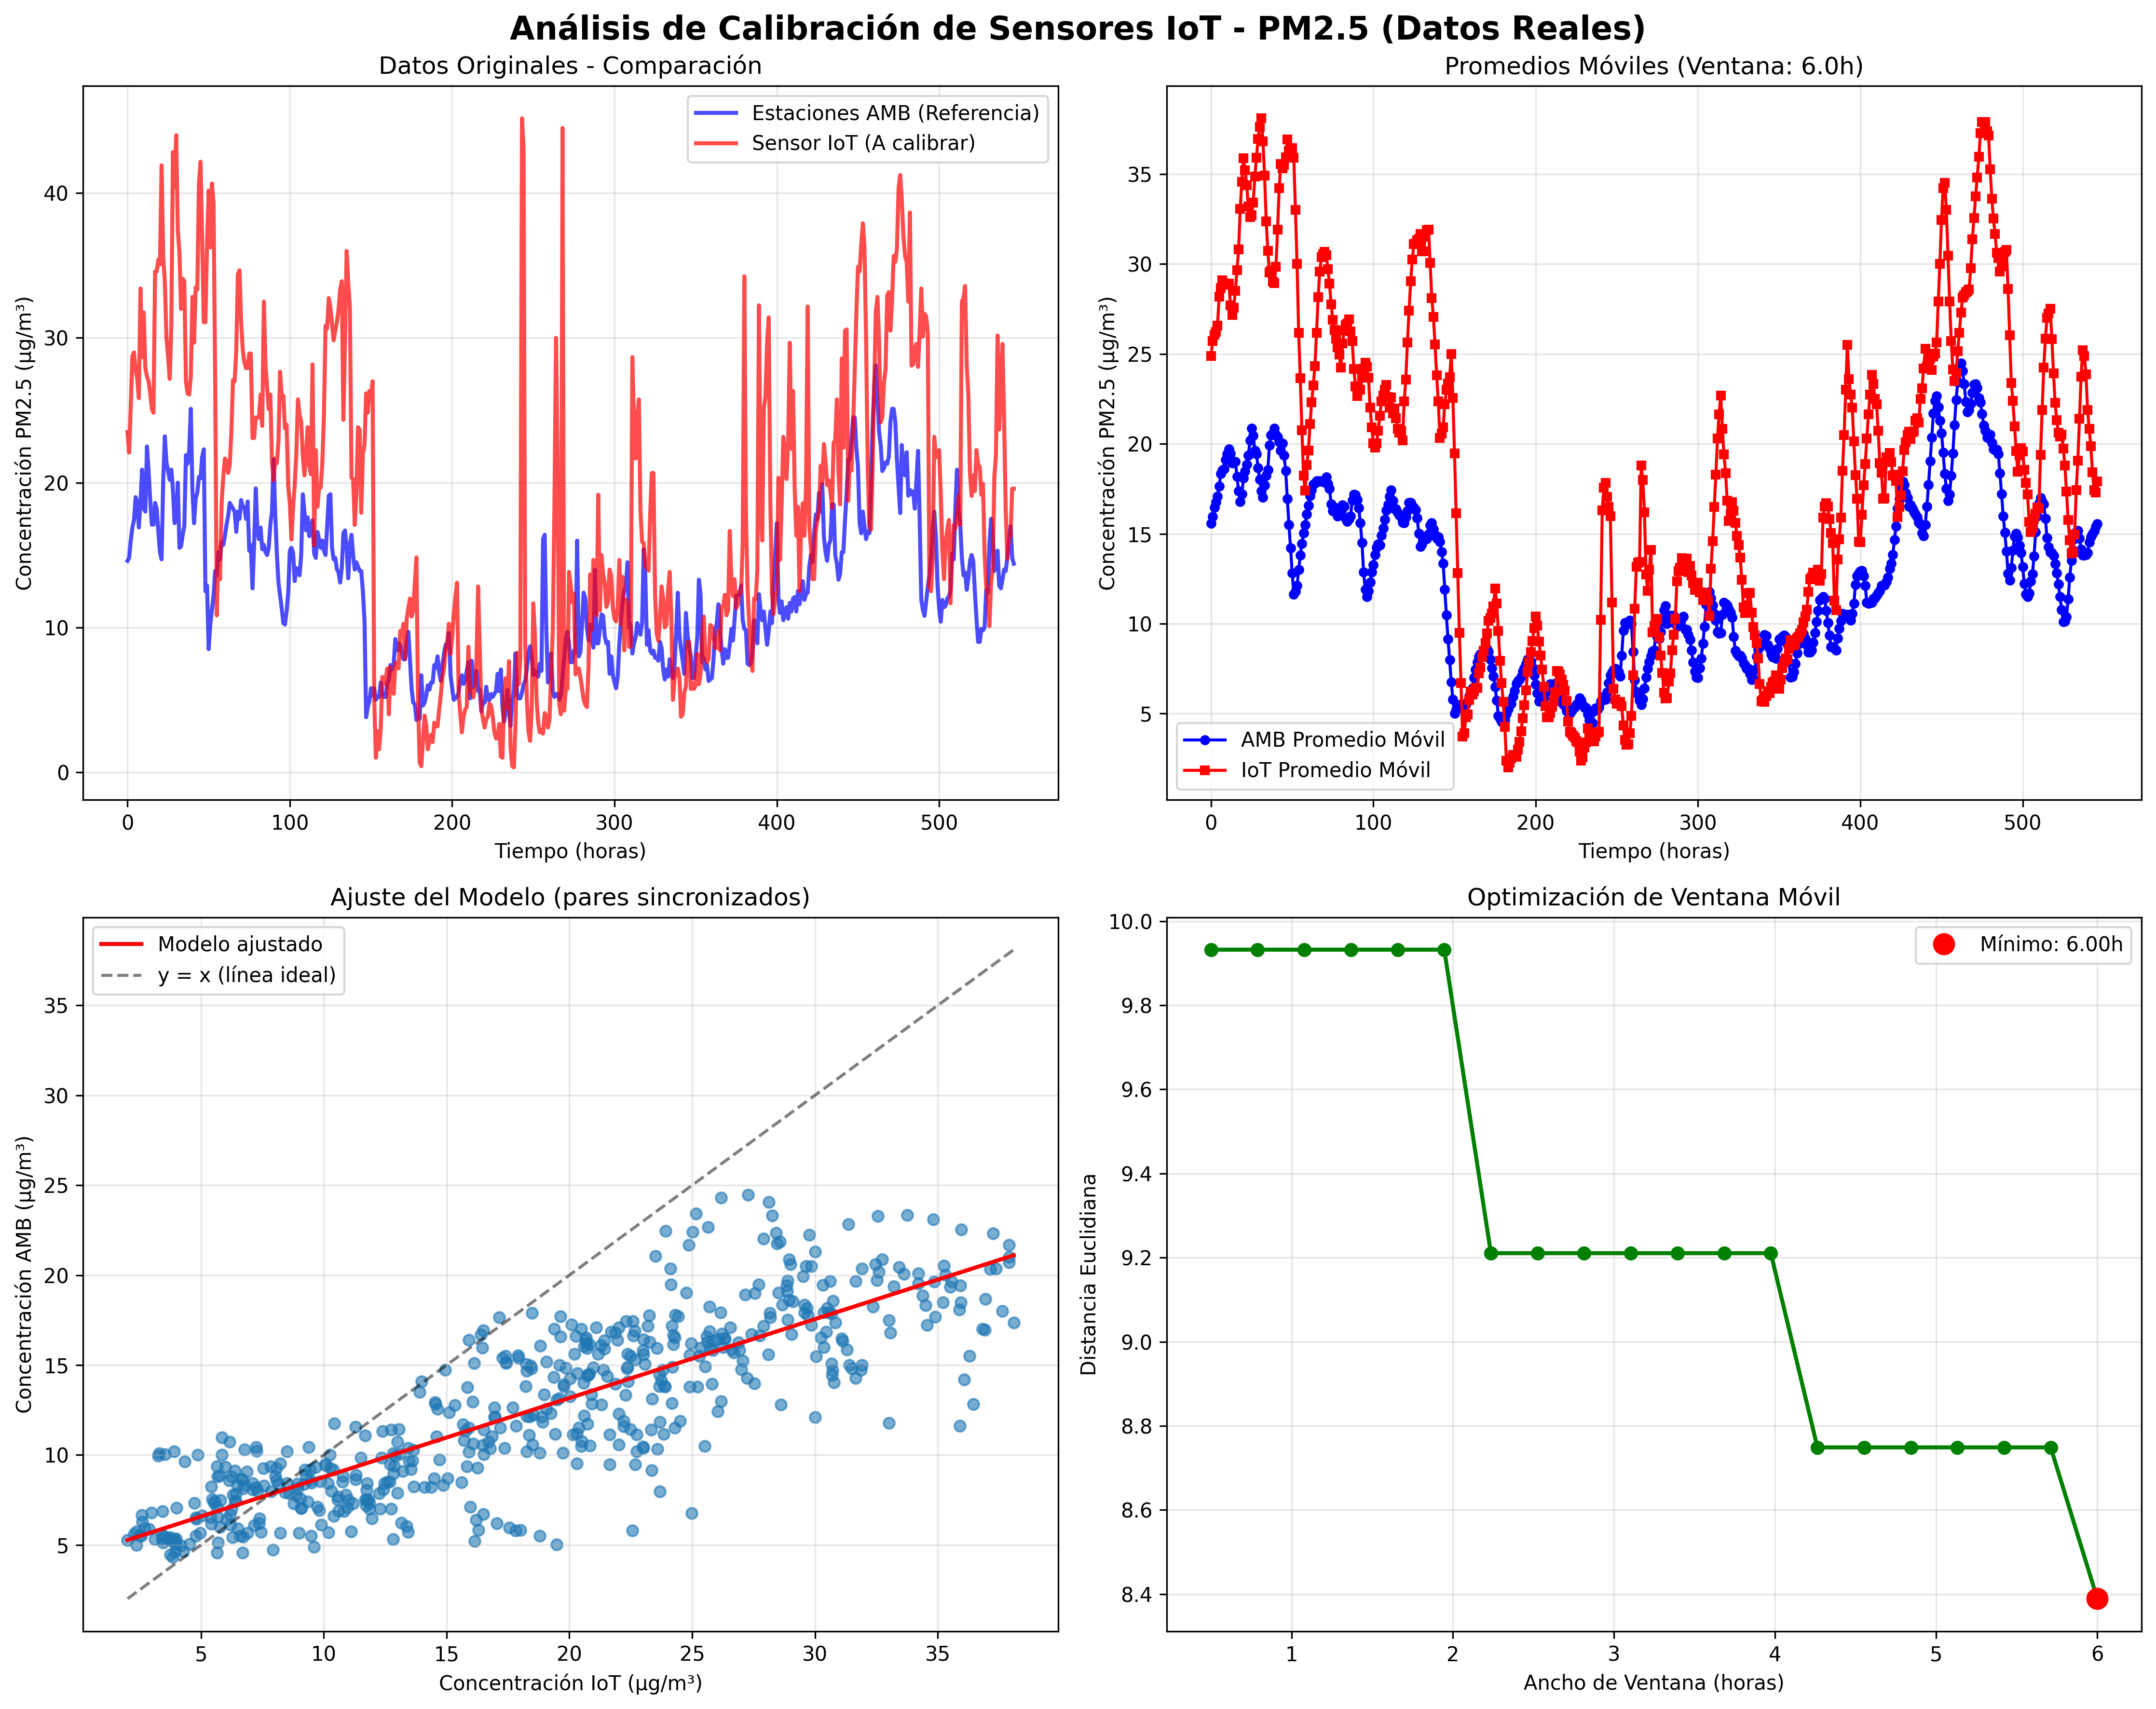
\includegraphics[width=0.95\textwidth]{../Asignaciones/TallerDistancias/resultados_datos_reales.png}
\caption{Análisis completo de calibración de sensores IoT PM2.5. (a) series temporales originales de referencia (azul) y sensor IoT (rojo). (b) promedios móviles con ventana óptima de 6.0 h. (c) ajuste lineal entre pares sincronizados mostrando la relación $f = 0.4389\,\hat{f} + 4.3893$. (d) optimización de ventana móvil con mínimo en 6.0 h (distancia = 8.3890).}
\label{FiguraResultados}
\end{figure}

\section{Conclusiones y Recomendaciones}
\label{Conclusiones}
Los resultados muestran que el uso de promedios móviles y un modelo lineal simple permite calibrar razonablemente un sensor IoT frente a una estación de referencia, con buen poder explicativo ($R^2\approx0.71$) y error cuadrático medio moderado. El modelo es válido dentro del rango de concentraciones observado para IoT entre 2.01 y 38.10~$\mu\mathrm{g}/\mathrm{m}^3$ bajo una tolerancia del 25\%.

Como trabajo futuro, se sugiere explorar modelos no lineales en presencia de saturaciones o sesgos, y analizar la sensibilidad a la selección de ventana y a diferentes estrategias de sincronización temporal.

\section{Referencias}
Basado en el Taller de Distancias del Prof. L. A. Núñez, Universidad Industrial de Santander. 

Código fuente y datos disponibles en: \texttt{taller\_distancias.py} y carpeta \texttt{DatosDistancias/}.

Para metodologías adicionales de calibración de sensores IoT, consultar:
\begin{itemize}
\item Zimmerman et al. (2018). \textit{A machine learning calibration model using random forests to improve sensor performance for lower-cost air quality monitoring}.
\item Metodología de distancias euclidianas aplicada según especificaciones del Taller de Distancias (2025).
\end{itemize}

\end{document}
